\subsection{Thermal sum}
\label{section: thermal sum}

When evaluating thermal integral, we will often encounter sums of the form
\begin{equation}
    \label{j func}
    j(\omega, \mu) = \frac{1}{2\beta} \sum_{\omega_n} 
    \ln\{\beta^2 [(\omega_n + i \mu) + \omega^2] \} + g(\beta),
\end{equation}
where the sum is over either the bosonic Matsubara frequencies $\omega_n = 2n \pi / \beta,\, n \in \mathbb{Z}$, or the fermionic ones, $\omega_n = (2n + 1) \pi /\beta ,\, n \in \mathbb{Z}$.
$\mu \in \R$ is a chemical potential.
$g$ may be a function of $\beta$, but we assume it is independent of $\omega$.
Thus, the factor $\beta^2$ could strictly be dropped, but it is kept to make the argument within the logarithm dimensionless.
We define the function
\begin{equation}
    \label{i func}
    i(\omega, \mu) = \frac{1}{\omega} \odv{\omega} j(\omega, \mu) 
    = \frac{1}{\beta} \sum_{\omega_n} \frac{1}{(\omega_n + i\mu)^2 + \omega^2}. 
\end{equation}

We will first work with the sum over bosonic Matsubara frequencies.
Assume $f(z)$ is an analytic function, except perhaps on a set of isolated poles $\{z_i\}$ located outside the real line.
We can exploit this using the properties of the Bose-distribution $n_B(z)$.
The Bose distribution is defined as 
\begin{equation}
    n_B(\omega) = \frac{1}{e^{\beta \omega} - 1}.
\end{equation}
This function obeys
\begin{equation}
    n_B(- i \omega) = -1 - n_B(i \omega).
\end{equation}
We can expand it around the Bose Matsubara frequencies on the imaginary line:
\begin{equation}
    i n_B[i (\omega_n + \epsilon)] = \frac{i}{e^{i\beta \epsilon + 2 \pi i n} - 1}
    = i [i\beta \epsilon + \Oh{(\epsilon)} ]^{-1} \sim  \frac{1}{\epsilon \beta}.
\end{equation}
This means that $in_B(i\omega)$ has a pole on all Matsubara-frequencies, with residue $1/\beta$.
Using this, we can rewrite the sum over Matsubara frequencies as a contour integral
\begin{equation*}
    \frac{1}{\beta} \sum_{\omega_n} f(\omega_n) 
    = \oint_\gamma \frac{\dd z}{2 \pi i} f(z) i n_B(i z),
\end{equation*}
where $\gamma$ is a contour that goes from $- \infty - i \epsilon$ to $+ \infty - i \epsilon$, crosses the real line at $\infty$, goes from $+ \infty - i \epsilon$ to $- \infty + i \epsilon$ before closing the curve.
The contour $\gamma$ and the new contours are illustrated in \autoref{fig:integral contours}.
This result exploits Cauchy's integral formula by letting the poles of $in_B(iz)$ at the Matsubara frequencies ``pick out'' the necessary residues.
The integral over $\gamma$ is equivalent to two integrals along $\R \pm i \epsilon$,
\begin{align}
    \nonumber
    \frac{1}{\beta} \sum_{\omega_n} f(\omega_n) 
    &= \left(
        \int_{\infty + i \epsilon}^{-\infty + i \epsilon} \frac{\dd z}{2 \pi} 
        + \int_{-\infty - i \epsilon}^{\infty - i \epsilon}\frac{\dd z}{2 \pi}
    \right) 
    f(z) n_B(i z),
    \\
    \nonumber
    & = \int_{-\infty - i \epsilon}^{\infty - i \epsilon}\frac{\dd z}{2 \pi}
    \left\{
        -f(-z) + \left[f(z) - f(-z)\right] n_B(iz)
    \right\} 
    \\
    \label{bosonic sum to integral}
    & = \int_{-\infty}^{\infty} \frac{\dd z}{2 \pi} f(z)
    +
    \int_{-\infty - i \epsilon}^{\infty - i \epsilon}\frac{\dd z}{2 \pi}
    \left[
        f(z) + f(-z)
    \right]
    n_B(iz).
\end{align}

\begin{figure}[ht]
    \centering
    \begin{subfigure}{0.4\textwidth}
        \centering
        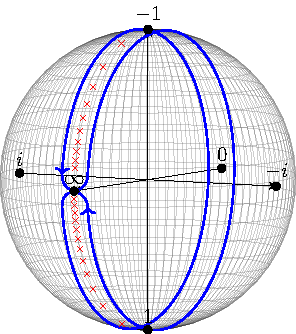
\includegraphics{thermal_field_theory/plots/integral_cont.pdf}        
    \end{subfigure}
    \begin{subfigure}{0.18\textwidth}
        \centering
        \begin{tikzpicture}
            \draw[-stealth] (0, 0) -- (1, 0);
        \end{tikzpicture}
        \end{subfigure}
    \begin{subfigure}{0.4\textwidth}
        \centering
        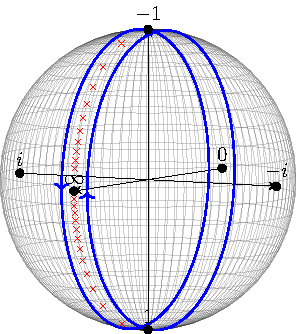
\includegraphics{thermal_field_theory/plots/integral_cont2.pdf}
    \end{subfigure} 
    \caption{The integral contour $\gamma$, and the result of deforming it into to contours close to the real line.
    The red crosses illustrate the poles of $n_B$.}
    \label{fig:integral contours}
\end{figure}

In the second line, we have changed variables $z \rightarrow -z$ in the first integral, and exploited the property $n_B(-i z) = -1 - n_B(iz)$.
In the last line, we use the assumption that $f(z)$ is analytic on the real line, and therefore also in a neighborhood of it. 
This allows us to shift the first integral back to the real line.
As $n_B(iz)$ is analytic outside the real line, the result of the second integral is the sum of residues of $f(z) + f(-z)$ in the lower half-plane.
The function
\begin{equation}
    f(z) 
    = \frac{1}{(z + i \mu)^2 + \omega^2} 
    = \frac{i}{2 \omega } 
    \left(
        \frac{1}{z + i(\mu + \omega)} - \frac{1}{z + i(\mu - \omega)}
    \right)
\end{equation}
obeys the assumed properties, as it has poles at
$z = - i (\mu \pm \omega)$, with residue $1 /( 2 \omega)$, so the function defined in \autoref{i func} may be written
\begin{equation}
    i(\omega, \mu) 
    = \frac{1}{2\omega}
    [1 + n_B(\omega - \mu) + n_B(\omega + \mu)].
\end{equation}

Using the antiderivative of the Bose distribution,
\begin{equation}
    \odv{\omega} \ln(1 - e^{-\beta \omega}) = \beta n_B(\omega),
\end{equation}
we get the final form of \autoref{j func}
\begin{equation}
    j(\omega, \mu) = \int \dd \omega'\, \omega' i(\omega', \mu)
    =  
    \frac{1}{2}\omega + \frac{1}{2\beta} 
    \left[
        \ln\left(1 - e^{-\beta(\omega - \mu)}\right)
        + \ln\left(1 - e^{-\beta(\omega + \mu)}\right)
    \right]
    + g'(\beta).
\end{equation}
The extra $\omega$-independent term $g'(\beta)$ is an integration constant.
We see there are temperature dependent terms, one due to the particle and one due to the anti-particle, and one due to the antiparticle, as they have opposite chemical potentials.

We now consider the sum over fermionic frequencies, which we for clarity denote $\tilde \omega_n$ in this chapter.
The procedure, in this case, is the same, except that we have to use a function with poles at the fermionic Matsubara frequencies.
This is done by the Fermi distribution, $n_F(z)$.
The Fermi distribution is
\begin{equation}
    n_F(\omega) = \frac{1}{e^{\beta \omega} + 1}.
\end{equation}
It obeys
\begin{align}
    &\odv{}{\omega} \ln(1 + e^{-\beta \omega}) = - \beta n_F(\omega), \\
    & n_F(- i\omega) = 1 - n_F(i\omega).
\end{align}
% The two distributions are related by
% \begin{equation}
%     2 n_B(i \omega; 2\beta) - n_B(i \omega; \beta)
%     = - n_F(i \omega; \beta ).
% \end{equation}
With this, the sum over fermionic Matsubara frequencies gives
\begin{align}
    \frac{1}{\beta} \sum_{\tilde \omega_n} f(\tilde \omega_n)
    & = \left(
        \int_{\infty + i \epsilon}^{-\infty + i \epsilon} \frac{\dd z}{2 \pi} 
        + \int_{-\infty - i \epsilon}^{\infty - i \epsilon}\frac{\dd z}{2 \pi}
    \right) 
    f(z) n_B(i z) \\
    & =
    \int_{-\infty}^{\infty} \frac{\dd z}{2 \pi} f(z)
    -
    \int_{-\infty - i \epsilon}^{\infty - i \epsilon}\frac{\dd z}{2 \pi}
    \left[
        f(z) - f(-z)
    \right]
    n_F(iz),
\end{align}
and 
\begin{equation}
    i(\omega, \mu) = \frac{1}{2 \omega} [1 - n_F(\omega - \mu) - n_F(\omega + \mu)].
\end{equation}
Using the antiderivative of the Fermi-distribution, we get
\begin{equation}
    j(\omega, \mu) 
    = \frac{1}{2} \omega 
    + \frac{1}{2 \beta }
    \left[
        \ln\left(1 + e^{-\beta(\omega - \mu)}\right)
        + \ln\left(1 + e^{-\beta(\omega + \mu)}\right)
    \right].
\end{equation}

